% =====================================================================================
% ICISN 2027 (Springer LNNS, llncs template). Max 10 pages, English.
% main.tex holds only the preamble, title and authors; the content lives in sections_icisn/
% (the first line of each file names its owner). Only Thuan edits main.tex.
%   Thuan   : Abstract, 1 Introduction, merging        files 0, 1
%   Khanh   : 2 Related Work, 3 Background, 7.1, 8     files 2, 3, 7_1, 8
%   Duc Anh : 4 Method (4.1-4.6), notation             file  4
%   Phat    : 5 Setup, 6 Results, 7.2-7.3              files 5, 6, 7_2, 7_3
% Rules: write in your own words (similarity <= 15%); every number must exist in the repo;
% never write "quantum advantage" or "state-of-the-art". Before submission: \showtodosfalse.
% Guide: HUONG_DAN_THANH_VIEN.md. Sources of the numbers:
%   main table   exps/scf/results/summary.md
%   ablation     results/scf_ablation.md  (python scripts/scf_ablation.py)
%   twin table   paper_acl/sections/results.tex (Table 1)
%   2x2 table    exps/qscf/results/summary.md   (after wave W07)
% =====================================================================================
\documentclass[runningheads]{llncs}
\usepackage[T1]{fontenc}
\usepackage{graphicx}
\usepackage{amsmath,amssymb}
\usepackage{booktabs}
\usepackage{multirow}
\usepackage{xcolor}
\usepackage{hyperref}
\renewcommand\UrlFont{\color{blue}\rmfamily}
\urlstyle{rm}

% ---- TODO notes: red, with the owner's name. \TODOT Thuan, \TODOK Khanh, \TODOD Duc Anh, \TODOP Phat ----
\newif\ifshowtodos \showtodostrue   % set to \showtodosfalse to hide every TODO
\DeclareRobustCommand{\TODOX}[2]{\ifshowtodos{\color{red}\textbf{[TODO #1:} #2\textbf{]}}\fi}
\DeclareRobustCommand{\TODOT}[1]{\TODOX{Thuan}{#1}}
\DeclareRobustCommand{\TODOK}[1]{\TODOX{Khanh}{#1}}
\DeclareRobustCommand{\TODOD}[1]{\TODOX{Duc Anh}{#1}}
\DeclareRobustCommand{\TODOP}[1]{\TODOX{Phat}{#1}}
\newcommand{\Tr}{\mathrm{Tr}}

\begin{document}

\title{Statistics-Calibrated Fusion for Exemplar-Free Class-Incremental Learning:
A Quantum Measurement and Its Classical Twin}
\titlerunning{Statistics-Calibrated Fusion for Exemplar-Free CIL}

% Springer requires FULL names; ORCID optional: \author{Thuan Pham\inst{1}\orcidID{0000-...} \and ...}
% If the review is double-blind, hide authors, institute and acknowledgments in the review version.
\author{Pham Van Vuong Thuan\inst{1} \and Le Dinh Quoc Khanh\inst{1} \and
Nguyen Thuan Phat\inst{1} \and Le Duc Anh\inst{1}}
\authorrunning{P. V. V. Thuan et al.}
\institute{University of Engineering and Technology, Vietnam National University, Hanoi, Vietnam\\
\email{\TODOT{school email of the corresponding author, e.g. ...@vnu.edu.vn}}}

\maketitle

% =====================================================================================
% Owner: Thuan. 150--250 words (currently ~210). Numbers: exps/scf/results/summary.md, exps/qscf/results/summary.md
\begin{abstract}
Exemplar-free class-incremental learning (CIL) methods built on pre-trained transformers store a mean and a
covariance for every class seen so far, yet use these statistics only to retrain the classifier and discard them
at prediction time. We propose Statistics-Calibrated Fusion (SCF), which keeps the trained classifier and adds a
second score computed from the stored statistics, rescaled by a label-free factor so that a single fusion weight
carries over across scores and datasets. The second score can be classical, a closed-form ridge classifier, or
quantum, a pretty-good measurement (PGM) over class density matrices built from the same statistics. On four
benchmarks with three seeds, SCF raises the final accuracy of the RSIAT baseline by 0.38 to 0.67 points, without
retraining the network or storing any data. Every quantum component is compared with a classical twin that
receives the same inputs: the PGM matches ridge ($-0.04$ points, 95\% CI $[-0.17,+0.08]$, 12 paired runs), as our
invariance results and the least-squares view of the PGM predict. The gain comes from complementary errors: the
classifier and the PGM disagree on 14\% of ImageNet-R test images, and fusion raises accuracy on both old and new classes, whereas
training-time changes trade one for the other. A pre-registered $2\times2$ experiment confirms this: SCF adds 0.38
and 0.44 points of average accuracy on classically and quantum-trained networks, while quantum training adds
nothing measurable once SCF is used.
\keywords{Class-incremental learning \and Exemplar-free \and Score fusion \and
Quantum state discrimination \and Pre-trained models}
\end{abstract}
      % Thuan
% Owner: Thuan. ~1.25 pages. Numbers: exps/scf/results/summary.md, results/scf_ablation.md,
% exps/qscf/results/summary.md, paper_acl/sections/analysis.tex (error analysis, 61-run frontier).
\section{Introduction}\label{sec:intro}
In class-incremental learning (CIL) a model learns new classes task after task and must classify every class
seen so far. In the \emph{exemplar-free} setting it may not keep images of past tasks, so whatever it remembers
about an old class has to fit in a compact summary. Methods built on pre-trained vision transformers have made
this setting practical~\cite{l2p,ease,ssiat}. A common recipe trains a light adapter on each task and stores one
mean and one covariance per class~\cite{zhang2023slca,ssiat,rsiat}. RSIAT~\cite{rsiat}, a strong recent
baseline, uses these statistics to correct feature drift and to retrain the classifier on Gaussian samples. Once
the classifier is aligned, however, the statistics play no further role: predictions come from the linear head
alone. Other methods do classify with the statistics, through nearest class means~\cite{zhou2024aper},
Mahalanobis distances~\cite{goswami2023fecam} or a ridge head~\cite{mcdonnell2023ranpac}, but they replace the
trained classifier instead of complementing it.

The same statistics are also a natural input for a quantum model. A class mean and covariance define a density
matrix, and classifying a feature among such states is a problem of quantum state discrimination, for which the
pretty-good measurement (PGM)~\cite{hausladen1994pgm} is a standard choice. Quantum components, however, are
usually judged by inserting them into a strong classical pipeline and reporting a gain of a few tenths of a
point, close to the pipeline's own run-to-run variation, and without a classical model that receives the same
inputs~\cite{bowles2024better,li2026qkd}. Whether the quantum part matters then remains open.

We address both points with \emph{Statistics-Calibrated Fusion} (SCF), shown in Fig.~\ref{fig:pipeline}. SCF
keeps the trained classifier and, at prediction time, adds a second score computed from the stored statistics:
a closed-form ridge classifier or the PGM over class density matrices. The second score is rescaled by a factor
computed from unlabelled training features of the current task, so one fusion weight, chosen once on ImageNet-R
and then frozen, transfers across scores and datasets. SCF needs no extra training of the network and no stored
images. We evaluate it under a protocol designed to resolve small effects: three seeds per benchmark, paired
comparisons with 95\% confidence intervals, every head evaluated on the same trained network, and decision rules
fixed before each experiment. Our contributions are:
\begin{itemize}
  \item \textbf{C1, SCF.} A training-free fusion of the classifier with a statistics-based score. It raises the
        final accuracy of RSIAT by $+0.38$ to $+0.67$ points on CIFAR-100, ImageNet-R, ImageNet-A and CUB-200,
        with the interval above zero on three of them (Table~\ref{tab:main}). The ablation shows that the
        calibration factor turns the mean gain of the ridge score from $+0.14$ into $+0.48$ points
        (Sect.~\ref{sec:ablation}).
  \item \textbf{C2, a quantum measurement with its classical twin.} Every quantum component, at training or at
        prediction time, is compared with a classical model on the same inputs (Table~\ref{tab:twin}). Inside SCF
        the PGM equals ridge ($-0.04$, $[-0.17,+0.08]$, 12 paired runs). Three propositions explain why: circuits
        after the encoding, shrinkage of the states and rescaling of the score cannot change the prediction
        (Sect.~\ref{sec:props}).
  \item \textbf{C3, why fusion helps.} The linear head and the PGM make different errors: they disagree on
        14\% of ImageNet-R test images, and each is right on a different part of them. Fusion therefore raises accuracy on old and new classes
        together, whereas every training-time change we tried trades one for the other (Sect.~\ref{sec:why}).
        A pre-registered $2\times2$ experiment confirms this: SCF adds $+0.38$ and $+0.44$ points of average
        accuracy on classically and quantum-trained networks, while quantum training adds $+0.09$,
        $[-0.08,+0.26]$, once SCF is used (Sect.~\ref{sec:qscf}).
\end{itemize}

\begin{figure}[t]
\centering
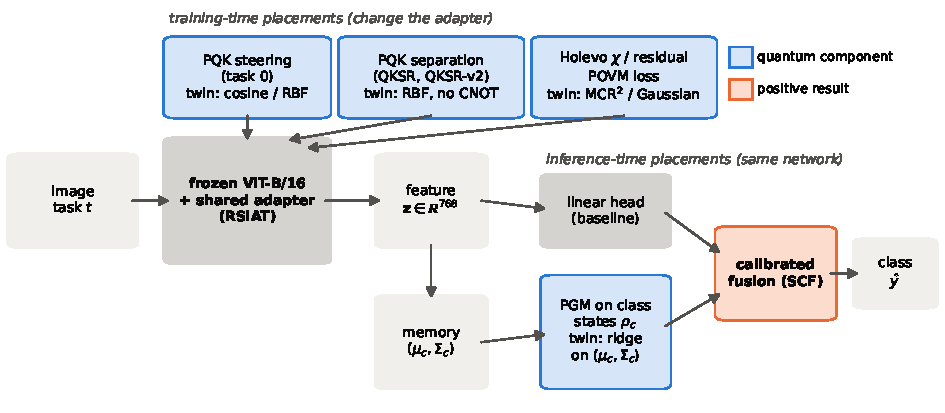
\includegraphics[width=\textwidth]{figures/pipeline.pdf}
\caption{\TODOD{Placeholder figure from the ACL version. Redraw it in the order of the Method section,
left to right: (1) training: image $\to$ ViT+adapter, PQK on the base task and QKSR on incremental tasks
(small, faded box); (2) memory $(\mu_c,\Sigma_c)$; (3) inference (main, highlighted box):
$z$ $\to$ linear head $\|$ (memory $\to\rho_c\to$ PGM, or ridge) $\to$ fusion with $\kappa$ $\to\hat y$.
You can edit \texttt{paper\_acl/make\_figures.py}, function \texttt{pipeline()}.}}
\label{fig:pipeline}
\end{figure}
  % Thuan
% Owner: Khanh. ~1 page. End every paragraph with an "Unlike these works, we ..." sentence.
\section{Related Work}\label{sec:related}
\paragraph{Class-incremental learning with pre-trained models.}
\TODOK{Prompt/adapter-based: L2P~\cite{l2p}, DualPrompt~\cite{dualprompt}, CODA-Prompt~\cite{codaprompt},
EASE~\cite{ease}, MOS~\cite{mos}, SSIAT~\cite{ssiat}, RSIAT~\cite{rsiat}. 3--4 sentences.}

\paragraph{Classifiers built from class statistics.}
\TODOK{MOST IMPORTANT PARAGRAPH. NCM/prototypes (SimpleCIL/APER~\cite{zhou2024aper}), FeCAM~\cite{goswami2023fecam},
RanPAC~\cite{mcdonnell2023ranpac}, SLCA~\cite{zhang2023slca}. Check the positioning table in KE\_HOACH\_NHOM.md
against the original papers. Closing sentence: these methods replace the classifier or retrain it; SCF keeps the
classifier and adds a statistics-based score at inference, calibrated without labels.}

\paragraph{Quantum machine learning and classical baselines.}
\TODOK{Projected quantum kernels~\cite{huang2021power,thanasilp2024concentration}, QCL~\cite{jiang2022qcl},
QKD~\cite{li2026qkd}, the benchmark of Bowles et al.~\cite{bowles2024better}; PGM~\cite{hausladen1994pgm}
and its least-squares equivalence~\cite{eldar2001srm}.}
       % Khanh
% Owner: Khanh. ~0.5 page. Sources: paper_acl/sections/task.tex, method.tex (4.1)
\section{Background}\label{sec:background}
\paragraph{Problem and metrics.}
Tasks $t=0,\dots,B-1$ bring disjoint label sets $\mathcal Y_t$; after task $t$ the model classifies all
classes $\mathcal C_t=\mathcal Y_0\cup\dots\cup\mathcal Y_t$, $C_t=|\mathcal C_t|$, without storing past images.
With $A_k$ the accuracy on $\mathcal C_k$ after task $k$,
\begin{equation}
  \bar A=\frac1B\sum_{k=0}^{B-1}A_k,\qquad A_B=A_{B-1}.
  \label{eq:metrics}
\end{equation}
\TODOK{Rewrite the paragraph above in your own words; add forgetting $F$ if used.}

\paragraph{Baseline: RSIAT.}
\TODOK{Frozen ViT-B/16~\cite{dosovitskiy2021vit} + shared adapter; features $z\in\mathbb R^{768}$;
cosine classifier $\ell_c(z)=s\cos(w_c,z)$ (the \emph{linear head}); memory $\mathcal M_t=\{(\mu_c,\Sigma_c)\}$;
drift correction; classifier alignment with Gaussian samples~\cite{zhang2023slca}. Closing sentence: $\mathcal M_t$
is \emph{already there}; SCF adds nothing to it.}
    % Khanh
% Owner: Duc Anh. ~2.4 pages. Sources: paper_acl/sections/method.tex, appendix.tex (A).
% The equations below are copied from the ACL version to keep the notation consistent; rewrite the text.
% Order follows the pipeline: training (base -> incremental, 4.1) -> memory -> inference (4.2-4.6).
% Focus on 4.2-4.6 (PGM + SCF). Keep 4.1 short (~0.4 page).
\section{Method}\label{sec:method}
\TODOD{Opening paragraph, 3--4 sentences, following the pipeline (Fig.~\ref{fig:pipeline}): quantum components can
enter at training time, when the adapter learns the base task and the later tasks (Sect.~\ref{sec:pqk}); however
it is trained, all that remains of the old classes is the memory $\mathcal M_t$; at inference we read $\mathcal M_t$
as quantum states and measure them with the PGM (Sect.~\ref{sec:states}--\ref{sec:pgm}), then combine it with the
linear head (Sect.~\ref{sec:scf}).}

\subsection{Quantum Kernels at Training Time}\label{sec:pqk}
% ~0.4 page. NOT a main contribution: it defines what is needed to read the twin table and the 2x2 table.
% Sources: paper_acl/sections/method.tex Sect. 4.2 (PQK), PIPELINE_cho_nhom.md Sect. 4.
A feature is mapped to $q=8$ angles $\theta(z)=\pi\tanh(W\,\mathrm{LN}(z)+b)$, loaded with $R_y$ rotations and
followed by $L=2$ layers of trainable $R_y$ rotations and a ring of CNOTs. Following~\cite{huang2021power}, two
features are compared through the one-qubit reduced density matrices $\rho_j$ of their states:
\begin{equation}
  k(z,z')=\exp\Big(-\gamma\sum_{j=1}^{q}\big\|\rho_j(z)-\rho_j(z')\big\|_F^2\Big).
  \label{eq:pqk}
\end{equation}
\TODOD{Rewrite the paragraph above.}

\paragraph{Base task.} \TODOD{1--2 sentences: $k$ replaces the cosine in the RSIAT steering loss; the circuit is
trained together with the adapter and frozen after task 0.}

\paragraph{Incremental tasks (QKSR).} \TODOD{1--2 sentences: penalise the mean $k(\mathrm{AE}(\mu_c^{\mathrm{old}}), z)$
between old-class means and new features, to separate new classes from old ones. Twins: RBF on the same 8 angles;
the same circuit without CNOTs. In the paper, ``QKSR'' means both the base-task and incremental-task parts are on.}

\TODOD{Transition to 4.2: these kernels only change how the adapter learns; results in Table~\ref{tab:twin} and
Table~\ref{tab:qscf}. However the network is trained, old classes survive only as $(\mu_c,\Sigma_c)$; the next
part uses exactly these statistics at inference.}


\subsection{Classes as Quantum States}\label{sec:states}
\TODOD{1--2 lead-in sentences: at inference, each class in $\mathcal M_t$ becomes a quantum state.}
Let $m_0$ and $s_0^2$ be the mean and the trace of the covariance of the task-0 features.
\begin{equation}
  v(z)=\begin{bmatrix}(z-m_0)/s_0\\1\end{bmatrix}\in\mathbb R^{769},\qquad \psi(z)=\frac{v(z)}{\|v(z)\|},
  \label{eq:lift}
\end{equation}
\begin{equation}
  \rho_c=\frac{\mathbb E_c[vv^{\top}]}{\mathbb E_c\|v\|^2},\qquad
  \mathbb E_c[vv^{\top}]=\begin{bmatrix}\tilde\Sigma_c+\tilde\mu_c\tilde\mu_c^{\top}&\tilde\mu_c\\
  \tilde\mu_c^{\top}&1\end{bmatrix}.
  \label{eq:state}
\end{equation}
\TODOD{Explain: $\psi$ is a 10-qubit state (769 padded to 1024); $\rho_c$ is computed from
$(\mu_c,\Sigma_c)$ only, needs no stored features, and follows the drift correction.}

\subsection{Pretty-Good Measurement}\label{sec:pgm}
\begin{equation}
  E_c=\frac1{C_t}\,\bar\rho_\delta^{-1/2}\rho_c\,\bar\rho_\delta^{-1/2},\quad
  \bar\rho_\delta=\frac1{C_t}\sum_{c}\rho_c+\delta I,\quad
  p(c\mid z)=\frac{\psi^{\top}E_c\psi}{\sum_{c'}\psi^{\top}E_{c'}\psi}.
  \label{eq:pgm}
\end{equation}
\TODOD{Explain the role of $\bar\rho_\delta^{-1/2}$ (compares class $c$ against all classes) and of $\delta$.}

\subsection{Classical Twin: Ridge on the Same Statistics}\label{sec:ridge}
\begin{equation}
  \Big(\sum_{c}(\Sigma_c+\mu_c\mu_c^{\top})+\lambda I\Big)W=[\mu_1,\dots,\mu_{C_t}],\qquad
  g^{\mathrm R}_c(z)=z^{\top}W_{:,c}.
  \label{eq:ridge}
\end{equation}
\TODOD{Stress: same input $\mathcal M_t$ as the PGM; in the spirit of RanPAC~\cite{mcdonnell2023ranpac}.}

\subsection{Statistics-Calibrated Fusion (SCF)}\label{sec:scf}
\begin{equation}
  \hat y=\arg\max_c\;\ell_c(z)+w\,\kappa\,g_c(z),\qquad
  \kappa=\overline{\mathrm{sd}_c\,\ell_c}\,\big/\,\overline{\mathrm{sd}_c\,g_c},
  \label{eq:scf}
\end{equation}
\TODOD{$g$ = $\log p(c\mid z)$ (PGM) or $g^{\mathrm R}$; $\mathrm{sd}_c$ = standard deviation over classes, averaged
over the training images of the current task; $\kappa$ needs no labels; $w$ frozen on the tuning group
(ridge 0.25, PGM 0.5).}

\subsection{What the Measurement Can and Cannot Do}\label{sec:props}
\begin{proposition}\label{prop:unitary}
For any unitary $U$ applied after the encoding, $p(c\mid z)$ is unchanged.
\end{proposition}
\begin{proposition}\label{prop:shrink}
Replacing every $\rho_c$ by $(1-\varepsilon)\rho_c+\varepsilon\bar\rho$, $\varepsilon\in[0,1)$, leaves
$\arg\max_c p(c\mid z)$ unchanged.
\end{proposition}
\begin{proposition}\label{prop:scale}
For any $a>0$ and class-independent $b(z)$, replacing $g_c$ by $a\,g_c+b$ leaves $\hat y$ in
Eq.~\eqref{eq:scf} unchanged.
\end{proposition}
\TODOD{A 2--3 line proof for each proposition (appendix.tex Sect. A). After each, one sentence on its practical
meaning: (1) training a circuit after the encoding is useless; (2) shrinking the states has no effect; (3) $w$ means
the same for every source and dataset, so it can be frozen. Also: the PGM coincides with the least-squares
measurement~\cite{eldar2001srm}, so we predict ridge $\approx$ PGM.}
        % Duc Anh
% Owner: Phat. ~0.5 page. Sources: paper_acl/sections/setup.tex, task.tex
\section{Experimental Setup}\label{sec:setup}
\TODOP{4 datasets: CIFAR-100~\cite{krizhevsky2009cifar} (10 tasks), ImageNet-R~\cite{hendrycks2021many} (10 tasks),
ImageNet-A~\cite{hendrycks2021nae} (10 tasks), CUB-200~\cite{wah2011cub} (20 tasks); seeds 1993, 2015, 2026;
data splits; ViT-B/16 IN-21K; GPU: NVIDIA RTX PRO 6000 Blackwell (Kaggle); paired comparisons + 95\% CI; $w$ frozen on ImageNet-R seed 1993;
every head is evaluated on the same network.}
         % Phat
% Owner: Phat. ~1.5 pages.
\section{Results}\label{sec:results}

\begin{table}[t]
\centering
\caption{Exemplar-free CIL, ViT-B/16-IN21K. Top: reported by~\cite{rsiat} on the authors' partitions (one run).
Bottom: our runs, mean $\pm$ SD over 3 seeds; $\Delta$: paired difference to RSIAT with 95\% CI.
\TODOP{Rewrite the caption; decide how many published rows to keep (the ACL version has 10).
Springer discourages \texttt{\textbackslash resizebox} and \texttt{\textbackslash tiny}: consider moving the $\Delta$ rows to a separate small table.}}
\label{tab:main}
\resizebox{\textwidth}{!}{%
\begin{tabular}{lcccccccc}
\toprule
& \multicolumn{2}{c}{CIFAR-100} & \multicolumn{2}{c}{ImageNet-R} & \multicolumn{2}{c}{ImageNet-A} & \multicolumn{2}{c}{CUB-200} \\
\cmidrule(lr){2-3}\cmidrule(lr){4-5}\cmidrule(lr){6-7}\cmidrule(lr){8-9}
Method & $\bar A$ & $A_B$ & $\bar A$ & $A_B$ & $\bar A$ & $A_B$ & $\bar A$ & $A_B$ \\
\midrule
SLCA~\cite{zhang2023slca} & 94.09 & 91.53 & 81.17 & 77.00 & 68.66 & 58.74 & 89.51 & 82.19 \\
RanPAC~\cite{mcdonnell2023ranpac} & 94.35 & 90.86 & 82.98 & 77.94 & 69.32 & 61.82 & 93.13 & 89.40 \\
SSIAT~\cite{ssiat} & 94.35 & 91.35 & 83.63 & 79.38 & 70.83 & 62.43 & 93.38 & 89.53 \\
RSIAT~\cite{rsiat} & 95.15 & 92.20 & 86.92 & 82.75 & 74.89 & 66.23 & 93.99 & 90.59 \\
\midrule
RSIAT (ours) & 95.02{\tiny$\pm$.21} & 92.03{\tiny$\pm$.19} & 87.11{\tiny$\pm$.49} & 82.55{\tiny$\pm$.05}
 & 74.26{\tiny$\pm$1.1} & 67.02{\tiny$\pm$1.1} & 93.53{\tiny$\pm$.79} & 88.47{\tiny$\pm$.31} \\
SCF, ridge & 95.22{\tiny$\pm$.20} & 92.41{\tiny$\pm$.21} & 87.42{\tiny$\pm$.46} & 83.03{\tiny$\pm$.24}
 & 75.12{\tiny$\pm$1.2} & 67.69{\tiny$\pm$0.9} & 93.54{\tiny$\pm$.88} & 88.85{\tiny$\pm$.22} \\
SCF, PGM & 95.23{\tiny$\pm$.22} & 92.34{\tiny$\pm$.16} & 87.50{\tiny$\pm$.43} & 83.07{\tiny$\pm$.42}
 & 74.89{\tiny$\pm$1.0} & 67.65{\tiny$\pm$1.3} & 93.50{\tiny$\pm$.84} & 88.57{\tiny$\pm$.30} \\
\midrule
$\Delta$ ridge & $+$.20 {\tiny[.12,.28]} & $+$.38 {\tiny[.08,.69]} & $+$.32 {\tiny[.12,.51]} & $+$.48 {\tiny[.02,.94]}
 & $+$.85 {\tiny[.62,1.08]} & $+$.67 {\tiny[$-$.20,1.54]} & $+$.02 {\tiny[$-$.24,.27]} & $+$.38 {\tiny[.16,.61]} \\
$\Delta$ PGM & $+$.22 {\tiny[.15,.28]} & $+$.31 {\tiny[.18,.43]} & $+$.39 {\tiny[.25,.53]} & $+$.52 {\tiny[$-$.41,1.45]}
 & $+$.63 {\tiny[$-$.10,1.36]} & $+$.62 {\tiny[$-$.08,1.32]} & $-$.03 {\tiny[$-$.18,.12]} & $+$.10 {\tiny[.05,.16]} \\
\bottomrule
\end{tabular}}
\end{table}

\paragraph{SCF raises final accuracy on all four benchmarks.}
\TODOP{Read Table~\ref{tab:main} and Fig.~\ref{fig:gain}: A$_B$ rises by +0.38 to +0.67 (ridge), the CI excludes 0
on 3/4; $\bar A$ does not rise on CUB-200. Position against the published numbers, noting the different data splits.}

\begin{figure}[t]
\centering
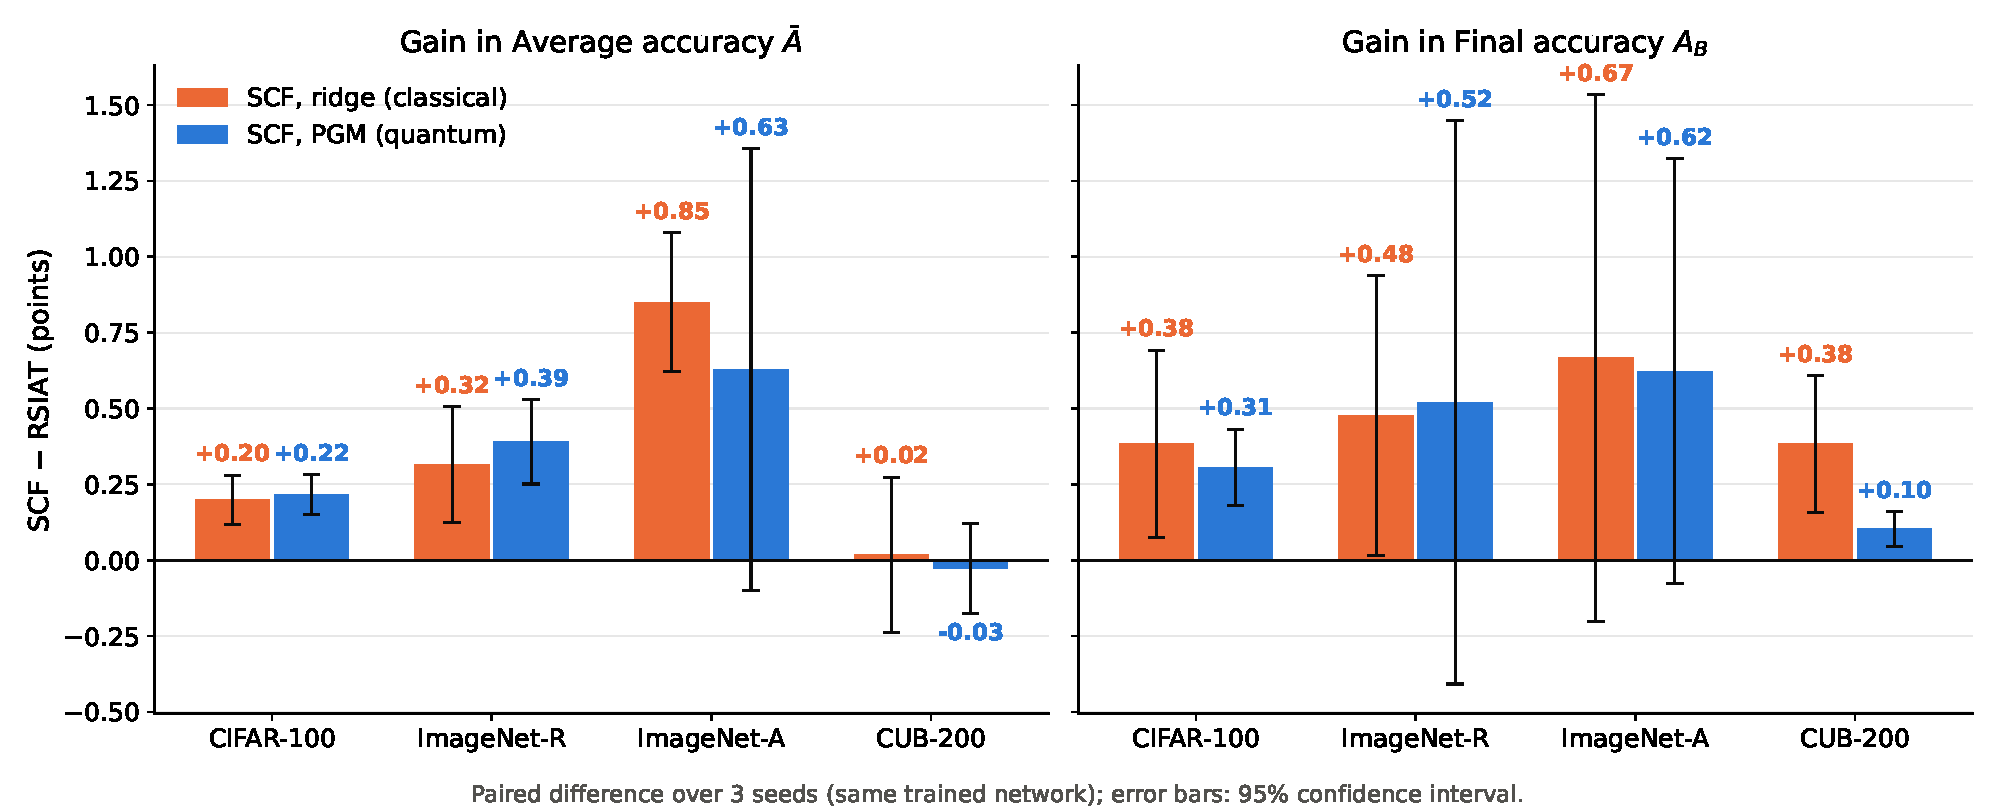
\includegraphics[width=\textwidth]{figures/scf_gain.pdf}
\caption{Paired gain of SCF over RSIAT (3 seeds, same network), 95\% CI. \TODOP{Rewrite the caption.}}
\label{fig:gain}
\end{figure}

\begin{table}[t]
\centering
\caption{Every quantum component against its classical twin (same inputs). $\Delta\bar A$ in points, paired
runs. R: ImageNet-R, A: ImageNet-A. \TODOP{Shorten/rewrite the caption; keep or drop the Holevo row.}}
\label{tab:twin}
\small
\begin{tabular}{lll r}
\toprule
Component & Comparison & $\Delta\bar A$ [95\% CI] & $n$ \\
\midrule
PQK, steering metric & PQK $-$ cosine, R & $+0.06$ [$-0.07$, $+0.18$] & 3 \\
PQK, separation (QKSR) & PQK $-$ RBF, R & $+0.07$ [$-0.01$, $+0.15$] & 3 \\
 & PQK $-$ no CNOT, R & $+0.04$ [$+0.04$, $+0.05$] & 3 \\
 & repaired $-$ original, R & $-0.07$ [$-0.11$, $-0.03$] & 3 \\
PQK, feature map & PQK ridge $-$ linear head, A & $-17.33$ [$-19.07$, $-15.59$] & 3 \\
Holevo objective & von Neumann $-$ MCR$^2$, R & $+0.06$ (screening) & 1 \\
PGM, stand-alone & PGM $-$ ridge, R+A & $+0.09$ [$-0.23$, $+0.40$] & 11 \\
PGM, fused (SCF) & PGM $-$ ridge, 4 datasets & $-0.04$ [$-0.17$, $+0.08$] & 12 \\
\bottomrule
\end{tabular}
\end{table}

\paragraph{The quantum score matches its classical twin.}
\TODOP{Read Table~\ref{tab:twin}: only one CI lies above 0 (+0.04); PGM = ridge, exactly as
Propositions~\ref{prop:unitary}--\ref{prop:scale} and the least-squares equivalence predict.}
       % Phat

\section{Analysis}\label{sec:analysis}
% Owner: Khanh. ~0.4 page. Source: paper_acl/sections/analysis.tex (7.2, 7.4)
\subsection{Why Fusion Helps}\label{sec:why}
\TODOK{Complementary errors: on ImageNet-R, PGM and the linear head disagree on 14\% of test images (linear right
5.8\%, PGM right 3.2\%, both wrong 5.4\%). Fig.~\ref{fig:frontier}: training-time changes only trade old classes for
new ones, fusion raises both. Do NOT reuse the old sentence ``uncalibrated sum +0.25/+0.44'' (different definition
from Table~\ref{tab:ablation}).}

\begin{figure}[t]
\centering
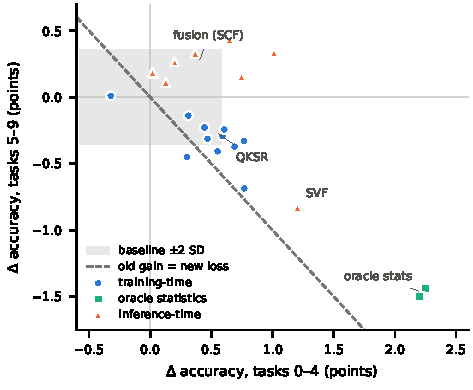
\includegraphics[width=0.6\textwidth]{figures/frontier.pdf}
\caption{Change of final accuracy on old (tasks 0--4) and new (tasks 5--9) halves, ImageNet-R seed 1993.
\TODOK{Rewrite the caption; shrink or drop the figure if pages run short.}}
\label{fig:frontier}
\end{figure}
         % Khanh
% Owner: Phat. ~0.4 page. Numbers: results/scf_ablation.md
\subsection{Ablation and Cost}\label{sec:ablation}
\begin{table}[t]
\centering
\caption{Ablation of SCF, final accuracy $A_B$ (mean over 3 seeds). Frozen weights: ridge $w=0.25$,
PGM $w=0.5$. \TODOP{Rewrite the caption; consider adding $\bar A$.}}
\label{tab:ablation}
\small
\begin{tabular}{lccccc}
\toprule
Variant & CIFAR-100 & ImageNet-R & ImageNet-A & CUB-200 & Mean \\
\midrule
Linear head (RSIAT) & 92.03 & 82.55 & 67.02 & 88.47 & 82.52 \\
Ridge alone & 91.41 & 80.02 & 65.71 & 87.40 & 81.14 \\
PGM alone & 91.32 & 80.11 & 65.06 & 85.90 & 80.60 \\
\midrule
Linear + ridge, no $\kappa$ ($w=1$) & 92.11 & 82.63 & 67.38 & 88.52 & 82.66 \\
Linear + PGM, no $\kappa$ ($w=1$) & 92.24 & 82.98 & 67.49 & 88.56 & 82.82 \\
\midrule
SCF ridge, $w=0.25$ (frozen) & 92.41 & 83.03 & 67.69 & 88.85 & 83.00 \\
SCF ridge, $w=1$ & 92.11 & 82.09 & 67.71 & 88.51 & 82.61 \\
SCF ridge, $w=4$ & 91.69 & 80.93 & 66.51 & 87.90 & 81.76 \\
SCF PGM, $w=0.5$ (frozen) & 92.34 & 83.07 & 67.65 & 88.57 & 82.91 \\
SCF PGM, $w=1$ & 92.34 & 82.96 & 67.67 & 88.55 & 82.88 \\
SCF PGM, $w=4$ & 91.90 & 81.83 & 66.62 & 87.77 & 82.03 \\
\bottomrule
\end{tabular}
\end{table}

\TODOP{3 sentences that match the numbers (see HUONG\_DAN Sect. 4a): (1) fusion beats each source alone, although
each source alone is worse than the linear head; (2) $\kappa$ is needed for ridge (without $\kappa$: +0.14 vs +0.48)
and helps less for PGM; (3) small-to-moderate $w$ (0.25--1) works, large $w$ hurts; $w$ is frozen on the tuning group.}

\TODOP{Cost (1 sentence or 1 row): run \texttt{scripts/scf\_cost.py}. CPU test numbers, $C=100$:
ridge +0.002\,ms/image, 0.6\,MB; PGM +0.9\,ms/image, $\sim$230\,MB. Replace with GPU numbers if available, naming the GPU.}
    % Phat
% Owner: Phat (W07 numbers run by Thuan). ~0.3 page. Numbers: exps/qscf/results/summary.md
\subsection{Quantum at Training Time plus SCF}\label{sec:qscf}
\begin{table}[t]
\centering
\caption{RSIAT or QKSR training $\times$ linear head or SCF, ImageNet-R seed 1993, 3 replicates
($\bar A$ / $A_B$, mean over 3 replicates). \TODOP{Rewrite the caption.}}
\label{tab:qscf}
\small
\begin{tabular}{lccc}
\toprule
Training & Linear head & SCF, ridge & SCF, PGM \\
\midrule
RSIAT & 87.39 / 82.50 & 87.76 / 82.75 & 87.76 / 82.85 \\
QKSR (PQK steering + separation) & 87.41 / 82.64 & 87.85 / 82.82 & 87.87 / 82.91 \\
\bottomrule
\end{tabular}
\end{table}

\TODOP{2--3 sentences, numbers from exps/qscf/results/summary.md (W07 done, 6/6 runs):
(1) SCF helps on both networks: SCF ridge $-$ linear, $\Delta\bar A$ = +0.38 [0.30, 0.46] on RSIAT and
+0.44 [0.36, 0.52] on QKSR;
(2) quantum training adds nothing once SCF is used: pre-registered test (QKSR+SCF ridge) $-$ (RSIAT+SCF ridge),
$\Delta\bar A$ = +0.09 [$-$0.08, +0.26], FAIL (CI contains 0); without SCF, QKSR $-$ RSIAT = +0.02 [$-$0.23, +0.27];
(3) so the gain comes from the inference-time fusion, not from the quantum kernels at training time.
Do NOT headline the PGM row (+0.12 [0.01, 0.22]): it was not the pre-registered test.}
        % Phat

% Owner: Khanh. ~0.5 page (including Limitations).
\section{Conclusion}\label{sec:conclusion}
\TODOK{Restate C1--C3 with numbers; lesson: always compare against a classical twin.}

\paragraph{Limitations.}
\TODOK{One baseline (RSIAT); data splits differ from the published numbers; small circuits ($\le$11 qubits)
simulated exactly; W07 covers only ImageNet-R with one seed; $\bar A$ does not rise on CUB-200; PGM memory is
$O(C\,D^2)$.}
    % Khanh

% Required by Springer (llncs v2.24, as in samplepaper.tex): Disclosure of Interests, before the references.
\begin{credits}
\subsubsection{\ackname} We thank Pham Thi Quynh Trang for supervising this work. Experiments were run on an
NVIDIA RTX PRO 6000 Blackwell GPU.

\subsubsection{\discintname}
The authors have no competing interests to declare that are relevant to the content of this article.
\end{credits}

\bibliographystyle{splncs04}
\bibliography{references}

\end{document}
